\documentclass[main.tex]{subfiles}
\begin{document}
\section{Попередній (ескізний) розрахунок ПНЧ}

\subsection{Мета розрахунку}

Метою даної роботи є придбання навиків розрахунку підсилювачів змінного струму, на разі підсилювача низької частоти (ПНЧ), і ескізного проектування.

\subsection{Теоретичні відомості}

Для виконання розрахунку необхідно знати основні характеристики підсилювачів змінного струму, принципи їх побудови та дії, методи розрахунку \cite{electronics_handbook}.

\subsection{Вихідні дані для розрахунку ПНЧ}

Вихідними даними для розрахунку є:
\begin{itemize}
    \item $P_\text{вих}$, Вт - потужність на виході підсилювача;
    \item $R_\text{н}$, Ом - опір навантаження;
    \item $U_\text{вх}$, В - напруга джерела вхідного сигналу;
    \item $R_{\text{дж}}$, Ом - внутрішній опір джерела вхідного сигналу;
    \item $\text{Вид схеми}$ : \\T - з трансформаторним зв'язком, \\Б - безтрансформаторна;
    \item $(f_{\text{н}} - f_{\text{в}})$,  Гц - нижня та верхня межі частот сигналу, що підсилюється;
\end{itemize}

\subsection{Теоретичні пояснення}

\subsection{Попередній (ескізний) розрахунок ПНЧ}

\subsubsection{Вихідні дані для розрахунку}

\begin{itemize}
    \item $P_\text{вих} = 2$ Вт - потужність на виході підсилювача;
    \item $R_\text{н} = 4$ Ом - опір навантаження;
    \item $U_\text{вх} = 15 \cdot 10^{-3}$ В = 0.015 В - напруга джерела вхідного сигналу;
    \item $R_{\text{дж}} = 330$ Ом - внутрішній опір джерела вхідного сигналу;
    \item $\text{Вид схеми} = T$ : \\T - з трансформаторним зв'язком, \\Б - безтрансформаторна;
    \item $(f_{\text{н}} - f_{\text{в}}) = 50 - 20000$ Гц - нижня та верхня межі частот сигналу, що підсилюється;
\end{itemize}

Вважаємо, що ПНЧ працює в стаціонарних умовах. Температура оточуючого середовища: 
\[
T_{min} = 15^\circ C; \quad T_{max} = 25^\circ C
\]
\subsubsection{Необхідно визначити:}

\begin{itemize}
    \item коефіцієнт підсилення ПНЧ за потужністю $K_P$;
    \item тип схеми вихідного (кінцевого) каскаду;
    \item типи транзисторів, каскадів підсилення (структурну схему ПНЧ);
    \item Орієнтовну електричну принципову схему ПНЧ;
\end{itemize}


\subsubsection{Порядок розрахунку}

\begin{enumerate}
\item \textbf{Знаходимо потужність вхідного сигналу} \newline
Найбільша потужність віддається в навантаження, коли його опір дорівнює
внутрішньому опору джерела. Тоді
\[
P_\text{вх} = \frac{U_\text{вх}^2}{4R_\text{дж}} = \frac{(0.015)^2}{4 \cdot 330} = \frac{0.000225}{1320} = 1.7 \cdot 10^{-7} \text{ Вт}
\]
де $R_{\text{дж}}$ - внутрішній опір джерела сигналу.

\item \textbf{Знаходимо потрібний коефіцієнт підсилення за потужністю}.

У загальному випадку рівність $R_{\text{вх}} = R_{\text{дж}}$ не виконується, а величина опору навантаження ПНЧ не дорівнює опору кінцевого каскаду. Тому на вході та виході
ПНЧ можуть бути застосовані узгоджувальні трансформатори, на яких буде
губитися частина потужності корисного сигналу. Крім того, в ПНЧ звичайно
застосовують регулятори рівня вихідного сигналу, що також викликає деяке
зниження потужності сигналу.

Керуючись цим, коефіцієнт підсилення за потужністю розраховують за
такою формулою:
\[
K_P = \frac{P_\text{вих}}{P_\text{вх} \cdot \eta_\text{Твх} \cdot \eta_\text{Твих} \cdot K_\text{рег}} = \frac{2}{1.7 \cdot 10^{-7} \cdot 0.75 \cdot 0.8 \cdot 0.4} = \frac{2}{4.08 \cdot 10^{-8}} = 4.9 \cdot 10^7
\]
де\\
$\eta_{\text{Твх}} = 0.75$ - ККД вхідного трансформатора, задається у межах (0.7 - 0.8);\\
$\eta_{\text{Твих}} = 0.8$ - ККД вихідного трансформатора, задається у межах (0.75 - 0.85);\\
$K_\text{рег} = 0.4$ - коефіцієнт передачі регулятора рівня сигналу, задається у межах (0.3 - 0.5);\\

Коефіцієнт підсилення за потужністю у децибелах:
\[
K_{P,\text{дБ}} = 10 \cdot \log_{10}(K_P) = 10 \cdot \log_{10}(4.9 \cdot 10^7) \approx 76.9 \text{ дБ}
\]

\item Попередньо вибираємо схему, тип підсилюючих приладів та
орієнтовну величину коефіцієнта підсилення за потужністю вихідного каскаду.
При цьому зважаємо на наступні рекомендації:
\begin{itemize}
    \item при розрахунковій потужності вихідного каскаду до 50 мВт доцільно
використовувати однотактну схему з малопотужним транзистором в режимі класу
А;
    \item за потужністю, що перевищує 50 мВт, треба застосовувати двотактну
схему, режим якої (клас АВ або В), потужність транзисторів (мала, середня чи
велика) визначаються з огляду на певне значення $P_{\text{вих}}$.
\end{itemize}

Тип транзистора вихідного каскаду вибираємо за величиною максимально
допустимої потужності, що розсіюється на його колекторі. Для цього знаходимо
потужність, яку транзистор повинен віддати у навантаження:
\[
P_\text{т} = \frac{P_\text{вих}}{\eta_\text{тр}} = \frac{2}{0.9} \approx 2.22 \text{ Вт}
\]
а потім знаходимо потужність, що споживається колекторним ланцюгом від джерела живлення:

\begin{itemize}
    \item для однотактного каскаду в режимі класу А:
\[
P_\text{к} = \frac{P_\text{т}}{\eta_\text{вих. каск}}
\]
    \item для двотактного каскаду в режимі класу АВ або В:
\[
P_{\text{к,AB}}
      =\frac{P_{\text{т}}\,(1-\eta_{\text{AB}})}{2\eta_{\text{AB}}}
      =\frac{2.22\,(1-0.60)}{2\cdot0.60}
      =\frac{2.22 \cdot 0.40}{1.20}
      =0.74\;\text{Вт}
\]
\end{itemize}
де $\eta_\text{вих. каск}$ - ККД вихідного каскаду (для однотактного каскаду приймається приблизно 0.4, а для двотактних - від 0.6 до 0.7).

У нашому випадку $P_\text{вих} = 2$ Вт > 50 мВт, тому в якості вихідного каскаду
вибираємо за умовами двотактну трансформаторну схему підсилення \cite{kolontaevsky_electronics}, для якої
\[
P_\text{т} = \frac{P_\text{вих}}{\eta_\text{тр}} = \frac{2}{0.9} \approx 2.22 \text{ Вт}
\]

За знайденим значенням $P_{k}$ вибираємо тип транзистора вихідного каскаду з довідника [4]. При цьому необхідно виконувати умови:
\[
P_\text{Кмакс} > P_\text{к}; f_{h21E} >> f_\text{в}
\]
де $P_\text{Кмакс}$ - максимальна допустима потужність, що розсіюється на колекторі обраного транзистора;\\
$f_{h21E}$ - гранична частота коефіцієнта передачі струму для вибраного типу транзистора в схемі з СЕ.

\begin{table}[H]
\centering
\caption{Основні параметри деяких транзисторів}
\label{tab:5.2}
\footnotesize
\begin{tabular}{|l|c|c|c|c|c|c|l|}
\hline
\textbf{Тип} & \textbf{Структура} & \textbf{$P_{\text{К}\max}$, мВт} & \textbf{$h_{21E}$} & \textbf{$f_{h21E}$, МГц} & \textbf{$U_{\text{K}\max}$, В} & \textbf{$I_{\text{К}\max}$, мА} & \textbf{Клас потужності} \\ 
\hline
КТ361Г   & p–n–p & 150  & 50–350   & 250 & 35 & 50   & Малої      \\ 
КТ3107Е  & p–n–p & 300  & 120-220  & 200 & 20 & 100  & Малої      \\ 
КТ315Г   & n-p-n & 150  & 50–350   & 250 & 35 & 100  & Малої      \\ 
\hline
КТ502В   & p–n–p & 500  & 40–120   & 5   & 60 & 300  & Середньої  \\ 
КТ503В   & n–p–n & 500  & 40–120   & 5   & 60 & 300  & Середньої  \\ 
\hline
КТ814А   & p–n–p & 1000 & $>$40    & 3   & 40 & 1500 & Великої    \\ 
КТ816А   & p–n–p & 1000 & $>$20    & 3   & 40 & 3000 & Великої    \\ 
КТ815А   & n–p–n & 1000 & $>$40    & 3   & 40 & 1500 & Великої    \\ 
КТ817А   & n–p–n & 1000 & $>$20    & 3   & 40 & 3000 & Великої    \\ 
\hline
\end{tabular}
\normalsize
\end{table}

Вибираємо транзистор КТ815А, який має максимальну потужність
\[ P_{K\max} = 1 \text{ Вт} > 0.74 \text{Вт} \] \[f_\text{h21E} = 3 \text{МГц} >> 20 \text{кГц} \]
У цьому випадку транзистор можна використовувати без додаткового охолодження.

\item Вибираємо схему каскадів попереднього підсилення.
Для попереднього підсилення, як правило, використовують підсилювачі з
СЕ.
У якості активного елемента застосуємо малопотужний транзистор КТ315Г \cite{boyko_electronics}
n-p-n типу, бо для вихідного каскаду також було обрано транзистор n-p-n типу.

\item Знаходимо орієнтовну кількість каскадів m та складаємо структурну
схему ПНЧ.

За певних умов можна вважати, що кожний каскад підсилювача за схемою з
СЕ забезпечує підсилення потужності приблизно на 20 дБ. Тоді
\[
m = \frac{K_{PdB}}{20} = \frac{76.9}{20} \approx 3.85
\]

Вибираємо значення m найближче до більшого цілого, тобто m = 4.
Структурна схема ПНЧ наведена на рис. ?, де цифрами 1-3 позначено каскади
попереднього підсилення, а цифрою 4 – вихідний (кінцевий) каскад.



\item На основі структурної схеми, з урахуванням вище наведених
міркувань складаємо орієнтовну принципову схему ПНЧ.

У цій схемі каскади попереднього підсилення виконано на транзисторах
VT1- VT3, а кінцевий – на транзисторах VT4,VT5. Резистор R9 є регулятором рівня вихідного сигналу. Конденсатор С10 – фільтр напруги живлення ПНЧ, а RС- фільтр (R14С7) забезпечує додаткову фільтрацію напруги живлення каскадів попереднього підсилення (забезпечує виконання умов електромагнітної сумісності). Величина опору резистора R14 зазвичай складає декілька десятків Ом.

\item Отримані в результаті попереднього розрахунку дані є основою для
остаточного розрахунку ПНЧ.
\end{enumerate}

\section{Остаточний розрахунок каскаду попереднього підсилення ПНЧ, виконаного за схемою з спільним емітером}

\subsection{Мета розрахунку}

Метою даної роботи є набуття навиків розрахунку транзисторних каскадів
попереднього підсилення низькочастотних сигналів змінного струму, у даному
разі звукових частот (ПНЧ).

\subsection{Теоретичні відомості}

Для виконання розрахунку необхідно знати основні характеристики
підсилювачів змінного струму, принцип дії та методи розрахунку транзисторних
каскадів попереднього підсилення ПНЧ, що працюють у режимі класу А [2,3].

\subsection{Вихідні дані}

Для остаточного розрахунку каскаду попереднього підсилення
транзисторного ПНЧ, що працює у режимі класу А та виконаний за схемою з СЕ,
вихідними даними є:
\begin{enumerate}
    \item $U_{\text{вих.т}}$, В -- напруга на виході (на навантаженні) каскаду;
    \item $R_{\text{н}}$, Ом -- опір навантаження (вхідний опір наступного каскаду);
    \item $E_{\text{К}}$, В -- напруга джерела живлення;
    \item $f_{\text{н}}$, Гц, $f_{\text{в}}$, кГц -- нижня та верхня межі діапазону частот сигналу, що підсилюється;
    \item $M_{\text{н}}$, $M_{\text{в}}$ -- допустимі значення коефіцієнтів частотних викривлень в області нижніх та верхніх частот.
\end{enumerate}

Вибір вихідних даних:
\begin{itemize}
    \item $U_{\text{вих.т}} = 0.35$ В -- напруга на виході (на навантаженні) каскаду;
    \item $R_{\text{н}} = 240$ Ом -- опір навантаження (вхідний опір наступного каскаду);
    \item $E_{\text{К}} = 14$ В -- напруга джерела живлення;
    \item $f_{\text{н}} = 100$ Гц, $f_{\text{в}} = 16$ кГц -- нижня та верхня межі діапазону частот сигналу, що підсилюється;
    \item $M_{\text{н}} = 1.10$, $M_{\text{в}} = 1.08$ -- допустимі значення коефіцієнтів частотних викривлень в області нижніх та верхніх частот.
\end{itemize}


\subsection{Теоретичні пояснення}

Остаточний розрахунок є основною частиною роботи при проектуванні ПНЧ. При його виконанні розраховують параметри елементів кожного каскаду, ланцюгів міжкаскадних зв’язків, режими роботи транзисторів. Розрахунок зазвичай виконують у послідовності, зворотній послідовності проходження сигналу в ПНЧ: спочатку розраховують елементи кінцевого каскаду, потім – передкінцевого, а далі – каскадів попереднього підсилення. Така послідовність обумовлена орієнтацією розрахунку на забезпечення на навантаженні ПНЧ заданої вихідної потужності за допустимих значень нелінійних та частотних викривлень сигналу.
Елементи схеми вибирають з урахуванням вимог стандартів до певних типів
компонентів. Так, резистори вибирають за номінальним значенням, найближчим
до розрахункової величини опору, та за величиною потужності, що розсіюється в
резисторі у робочому режимі. Конденсатори вибирають за номінальним
значенням ємності, найближчим до розрахункової величини, та за величиною
робочої напруги. Номінальні значення опорів резисторів та ємностей конденсаторів (між
іншим, як і номінальні значення параметрів будь-яких стандартних елементів)
відповідають стандартним рядам, що, як правило, є десятковими рядами N геометричної прогресії зі знаменником $q_{N} = \sqrt[N]{10}$ , де N – кількість значень ряду.
Деякі ряди номінальних значень наведені у табл. ?.

\begin{table}[H]
\centering
\caption{Ряди номінальних значень}
\label{tab:standard_values}
\begin{tabular}{|p{4cm}|p{4cm}|p{2.5cm}|}
\hline
\textbf{Індекс ряду} & \textbf{Позиції ряду} & \textbf{Допустиме відхилення від номінальної величини, \%} \\
\hline
E6 & 1,0; 1,5; 2,2; 3,3; 4,7; 6,8; & $\pm$ 20 \\
\hline 
E12 & 1,0; 1,2; 1,5; 1,8; 2,2; 2,7; 3,3; 3,9; 4,7; 5,6; 6,8; 8,2 & $\pm$ 10 \\
\hline
E24 & 1,0; 1,1; 1,2; 1,3; 1,5; 1,6; 1,8; 2,0; 2,2; 2,4; 2,7; 3,0; 3,3; 3,6; 3,9; 4,3; 4,7; 5,1; 5,6; 6,2; 6,8; 7,5; 8,2 & $\pm$ 5 \\
\hline
\end{tabular}
\end{table}

Числу в індексі ряду відповідає кількість позицій ряду: так ряд Е24 має 24
номінальних значення у проміжку від 1 до 10 (більша кількість при допустимому
відхиленні ± 5\% не потрібна).

Будь-яке номінальне значення ряду може бути помножене на множник 10 m.
Множники та їх позначення наведені в табл.6.3 (може бути, наприклад,
6,8 Ом; 68 Ом; 680 Ом; 6,8 кОм; 68 кОм; 6,8 мкФ; 0,68 нФ; 6800 пФ та ін.).

\begin{table}[H]
\centering
\caption{Множники номінальних значень}
\label{tab:multipliers}
\footnotesize
\begin{tabular}{|c|c|c|c|c|c|}
\hline
Множник $10^m$ & Приставка & Опір(назва) & Опер(Позначення) & Ємність(назва) & Ємність(Позначення) \\
\hline
$10^{9}$ & гіга & гігаом & ГОм & & \\
$10^{6}$ & мега & мегаом & МОм & & \\
$10^{3}$ & кіло & кілоом & кОм & & \\
$1$ & &         & Ом & фарада & Ф \\
$10^{-3}$ & мілі- & міліом & 1 мОм & & \\
$10^{-6}$ & мікро & & & мікрофарада & мкФ \\
$10^{-9}$ & нано & & & нанофарада & нФ \\
$10^{-12}$ & піко & & & пікрофарада & пФ \\
\hline
\end{tabular}
\normalsize
\end{table}

Номінальні значення деяких елементів, особливо застарілої розробки,
можуть відповідати іншим рядам.
Деякі найрозповсюджені типи резисторів, що виробляються для
електронних пристроїв, наведено в табл. 6.4, а конденсаторів – в табл. 6.5.
Примітки до табл. 6.5:
\begin{itemize}
    \item Якщо розрахункова величина ємності більша за максимальне номінальне
значення конденсаторів даного типу, то необхідне значення ємності забезпечують
за рахунок паралельного вмикання конденсаторів;
    \item Якщо розрахункова величина робочої напруги більша за номінальне
значення напруги конденсатора, то використовують послідовне вмикання
конденсаторів.
\end{itemize}

\begin{table}[H]
\centering
\caption{Постійні резистори}
\label{tab:resistor_types}
\footnotesize
\begin{tabular}{|p{3cm}|p{3cm}|p{3cm}|}
\hline
\textbf{Тип резистора} & \textbf{Діапазон опорів} & \textbf{Номінальна потужність, Вт} \\
\hline
МЛТ & 1 Ом - 3,01 МОм & 0,125 \\
 & 1 Ом - 5,01 МОм & 0,25; 0,5 \\
 & 1 Ом - 10 МОм & 1; 2 \\
\hline
C2 - 33 & 1 Ом - 3,1 МОм & 0,125 \\
        & 1 Ом - 5,1 МОм & 0,25 \\
        & 0,11 Ом - 5,1 МОм & 0,5 \\
        & 1 Ом - 10 МОм & 1 \\
        & 1 Ом - 22 МОм & 2 \\
\hline
\end{tabular}
\normalsize
\end{table}

\begin{table}[H]
\centering
\caption{Конденсатори постійної ємності}
\label{tab:6.5}
\tiny
\renewcommand{\arraystretch}{1.1}
\begin{tabular}{|c|c|c|c|c|c|}
\hline
\multirow{2}{*}{\textbf{Напруга}} 
& \multicolumn{5}{c|}{\textbf{Ном. ємність, мкФ}} \\ \cline{2-6}
& \textbf{К50--7} 
& \textbf{К50--35} 
& \textbf{К50--18} 
& \textbf{К10--17} 
& \textbf{К73--17} \\ 
\hline
6,3  & 20; 30; 50; 100; 200; 500 
     & 220 000             
     &                   
     &                   
     &                   \\ \hline
10   &                   
     & 10; 20; 30; 50; 100; 200; 500; 1000; 2000; 5000 
     & 100 000             
     &                   
     &                   \\ \hline
16   &                   
     & 5; 10; 20; 30; 50; 100; 200; 300; 1000; 2000; 5000 
     & 22 000; 68 000; 100 000 
     &                   
     &                   \\ \hline
25   &                   
     & 2; 5; 10; 20; 30; 50; 100; 200; 500; 1000; 2000; 5000 
     & 15 000; 33 000; 100 000 
     &                   
     &                   \\ \hline
50   &                   
     & 2; 5; 10; 20; 30; 50; 100; 200; 500; 1000; 2000; 5000 
     & 4 700; 10 000; 15 000; 22 000 
     & 0,001; 0,01; 0,022; 0,056                  
     &                   \\ \hline
63   &                   
     &                   
     & 
     &  
     & 0,22; 0,33; 0,47; 0,68; 1; 1,5; 2,2; 3,3; 4,7 \\ \hline
100  &                  
     & 0,5; 1; 2,5; 10; 20; 50;                  
     & 2200, 4700, 10000
     & 
     & \\ \hline
160  & 2; 50; 100; 200; 500                   
     & 1; 2; 5; 10; 20                   
     &  
     &  
     & 1,5; 2,2            \\ \hline
250  & 10; 20; 50; 100; 200                   
     &                   
     & 1000; 4700
     &                    
     & 0,047; 0,068; 0,1; 0,15; 0,22; 0,33; 0,47; 0,68; 1 \\ \hline
300  & 5; 10; 20; 50; 100; 200                
     &                   
     & 
     &                   
     &                   \\ \hline
350  & 10; 20; 50; 100                   
     &                   
     &  
     &                   
     &                   \\ \hline
450  & 10; 20; 50; 100                   
     &                   
     & 
     &                   
     &                   \\ \hline
\end{tabular}
\normalsize
\end{table}


\subsection{Остаточний розрахунок каскаду попереднього підсилення ПНЧ, з СЕ}

\subsubsection{Вихідні дані}

У результаті попереднього розрахунку було складено схему ПНЧ, в яку входять декілька однотипних каскадів попереднього підсилення з СЕ. 

Виконаємо розрахунок каскаду попереднього підсилення, схема електрична принципова якого наведена на рис. 6.1, за такими вихідними даними (загалом отримуються у результаті попереднього розрахунку):

\begin{itemize}
    \item Напруга на виході $U_{\text{вих.т}} = 0.35$ В;
    \item Опір навантаження $R_{\text{н}} = 240$ Ом;
    \item Напруга джерела живлення $E_{\text{К}} = 14$ В;
    \item Нижня межа діапазону частот сигналу, що підсилюється $f_{\text{н}} = 100$ Гц;
    \item Верхня межа діапазону частот сигналу, що підсилюється $f_{\text{в}} = 16$ кГц;
    \item Допустимі значення коефіцієнтів частотних викривлень в області нижніх та верхніх частот $M_{\text{н}} = 1.10$, $M_{\text{в}} = 1.08$.
\end{itemize}

Як і для попереднього розрахунку, вважаємо, що ПНЧ працює у стаціонарних умовах.

\subsubsection{Необхідно визначити}

\begin{enumerate}
    \item Тип транзистора VT1 (уточнити правильність вибору типу);
    \item Режими роботи транзистора VT1;
    \item Опори резисторів дільника: $R_1$, $R_2$;
    \item Опір резистора колекторного навантаження $R_3$;
    \item Опір резистора емітерного навантаження $R_4$;
    \item Ємність розділяючих конденсаторів $C_1$, $C_2$;
    \item Ємність конденсатора в ланцюгу емітера $C_3$;
    \item Гарантовані значення коефіцієнтів підсилення каскаду за струмом $K_I$, напругою $K_u$ та потужністю $K_p$
\end{enumerate}

При побудові схеми каскаду будемо використовувати елементи з допустимим відхиленням ± 5\% та номінальними значеннями, найближчими до розрахункових.
\begin{figure}[ht]
\centering
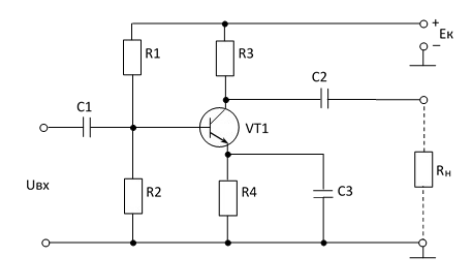
\includegraphics[width=0.8\textwidth]{images/cascad_ce.png}
\caption{Каскад підсилення з спільним емітером. Схема електрична принципова}
\label{fig:cascad_ce}
\end{figure}

\subsubsection{Порядок розрахунку}

\begin{enumerate}
\item \textbf{Тип транзистора VT1 (уточнюємо правильність попереднього вибору)} \newline
За вихідними даними, розрахуємо параметри для перевірки транзистора:

1) Визначаємо амплітуду вихідного струму:
    \[I_{\text{вих.m}} = \frac{U_{\text{вих.т}}}{R_{\text{н}}} = \frac{0.35\text{ В}}{240\text{ Ом}} \approx 1.46\text{ мА}\]

2) Для підсилювача класу А струм колектора у робочій точці повинен бути не менше ніж удвічі більше амплітуди вихідного струму:
    \[I_{\text{к0}} \geq 2 \cdot I_{\text{вих.m}} = 2 \cdot 1.46 \approx 2.92\text{ мА}\]

    Приймаємо \(I_{\text{к0}} = 3\text{ мА}\)

3) Напруга колектор-емітер у робочій точці:
    \[U_{\text{ке0}} \approx \frac{E_{\text{к}}}{2} = \frac{14\text{ В}}{2} = 7\text{ В}\]

4) Потужність, що розсіюється на колекторі:
    \[P_{\text{к}} = U_{\text{ке0}} \cdot I_{\text{к0}} = 7\text{ В} \cdot 3\text{ мА} = 21\text{ мВт}\]

5) Перевіряємо параметри КТ315Г:
    - \(P_{\text{кmax}} = 150\text{ мВт} > 21\text{ мВт}\)
    - \(f_{h21E} = 250\text{ МГц} \gg 16\text{ кГц}\)
    - \(I_{\text{кmax}} = 100\text{ мА} > 3\text{ мА}\)
    - \(U_{\text{кmax}} = 35\text{ В} > 14\text{ В}\)
    - \(h_{21E} = 50 \div 350\) достатньо для потрібного підсилення

Висновок: Попередній вибір транзистора КТ315Г є правильним, його параметри повністю задовольняють вимогам каскаду попереднього підсилення.

\item \textbf{Режими роботи транзистора VT1} \newline

В результаті попередніх розрахунків ми визначили, що струм колектора в робочій точці $I_{\text{к0}} = 3$ мА, а напруга колектор-емітер 

\[U_{\text{ке0}} = 7\text{ В}.\]

Визначаємо струм бази в робочій точці:
\[I_{\text{б0}} = \frac{I_{\text{к0}}}{h_{21E\text{,min}}} = \frac{3\text{ мА}}{50} = 0.06\text{ мА} = 60\text{ мкА}\]

Напруга база-емітер для кремнієвого транзистора:
\[U_{\text{бе0}} \approx 0.65\text{ В}\]

Для забезпечення температурної стабільності каскаду, визначимо значення коефіцієнта термостабілізації, яке повинно бути в діапазоні від 1 до 5. Приймаємо:
\[S = 2\]

Напруга на емітерному резисторі для забезпечення стабільності режиму роботи:
\[U_{\text{е0}} = \frac{I_{\text{к0}} \cdot h_{21E\text{,мин}}}{S \cdot (h_{21E\text{,мин}} - 1)} \cdot U_{\text{бе0}} \approx \frac{3 \cdot 10^{-3} \cdot 50}{2 \cdot 49} \cdot 0.65 \approx 1\text{ В}\]

Напруга на колекторному резисторі:
\[U_{R3} = E_{\text{к}} - U_{\text{ке0}} - U_{\text{е0}} = 14 - 7 - 1 = 6\text{ В}\]

Отже, режими роботи транзистора VT1:
\[I_{\text{к0}} = 3\text{ мА}\]
\[I_{\text{б0}} = 60\text{ мкА}\]
\[U_{\text{ке0}} = 7\text{ В}\]
\[U_{\text{бе0}} = 0.65\text{ В}\]
\[U_{\text{е0}} = 1\text{ В}\]

\item \textbf{Опори резисторів дільника: $R_1$, $R_2$} \newline

Для розрахунку резисторів дільника напруги спочатку визначимо напругу на базі транзистора:
\[U_{\text{б0}} = U_{\text{е0}} + U_{\text{бе0}} = 1\text{ В} + 0.65\text{ В} = 1.65\text{ В}\]

Для забезпечення стабільної роботи транзистора струм дільника обираємо приблизно рівним струму бази:
\[I_{\text{діл}} \approx I_{\text{б0}} = 60\text{ мкА}\]

Розраховуємо опори резисторів дільника:
\[R_2 = \frac{U_{\text{б0}}}{I_{\text{діл}}} = \frac{1.65\text{ В}}{60\text{ мкА}} = 27.5\text{ кОм}\]

Вибираємо зі стандартного ряду E24: $R_2 = 27\text{ кОм}$

\[R_1 = \frac{E_{\text{к}} - U_{\text{б0}}}{I_{\text{діл}}} = \frac{14\text{ В} - 1.65\text{ В}}{60\text{ мкА}} = 205.8\text{ кОм}\]

Вибираємо зі стандартного ряду E24: $R_1 = 180\text{ кОм}$

Перевіримо напругу на базі при обраних номіналах:
\[U_{\text{б}} = E_{\text{к}} \cdot \frac{R_2}{R_1 + R_2} = 14\text{ В} \cdot \frac{27\text{ кОм}}{180\text{ кОм} + 27\text{ кОм}} = 14 \cdot \frac{27}{207} \approx 1.826\text{ В}\]

Це значення близьке до розрахункового 1.65 В і забезпечить необхідний режим роботи.

\item \textbf{Опір резистора колекторного навантаження $R_3$} \newline

Розраховуємо опір резистора колекторного навантаження за законом Ома:
\[
R_3 = \frac{U_{R3}}{I_{\text{к0}}} = \frac{6\text{ В}}{3\text{ мА}} = 2\text{ кОм}
\]

Вибираємо зі стандартного ряду E24: $R_3 = 2.0\text{ кОм}$

Перевіряємо потужність, що розсіюється на резисторі:
\[
P_{R3} = U_{R3} \cdot I_{\text{к0}} = 6\text{ В} \cdot 3\text{ мА} = 18\text{ мВт}
\]

Ця потужність значно менша за номінальну потужність резистора МЛТ-0.125 (125 мВт), тому обираємо резистор $R_3 = 2.0\text{ кОм}$ (МЛТ-0.125).

\item \textbf{Опір резистора емітерного навантаження $R_4$} \newline

Розраховуємо опір резистора емітерного навантаження за законом Ома:
\[
R_4 = \frac{U_{\text{е0}}}{I_{\text{к0}}} = \frac{1\text{ В}}{3\text{ мА}} = 333.33\text{ Ом}
\]

Вибираємо зі стандартного ряду E24: $R_4 = 330\text{ Ом}$

Перевіряємо потужність, що розсіюється на резисторі:
\[
P_{R4} = U_{\text{е0}} \cdot I_{\text{к0}} = 1\text{ В} \cdot 3\text{ мА} = 3\text{ мВт}
\]

Ця потужність значно менша за номінальну потужність резистора МЛТ-0.125 (125 мВт), тому обираємо резистор $R_4 = 330\text{ Ом}$ (МЛТ-0.125).

\item \textbf{Ємність розділяючих конденсаторів $C_1$, $C_2$} \newline

Для розрахунку ємності розділяючих конденсаторів визначимо спочатку необхідні опори.

Для вхідного конденсатора $C_1$:
Вхідний опір каскаду можна розрахувати як:
\[R_{\text{вх}} \approx (R_1 \parallel R_2) \parallel (h_{21E,\text{мин}} \cdot R_4)\]

де $(R_1 \parallel R_2)$ - опір паралельного з'єднання резисторів дільника:
\[(R_1 \parallel R_2) = \frac{R_1 \cdot R_2}{R_1 + R_2} = \frac{180\text{ кОм} \cdot 27\text{ кОм}}{180\text{ кОм} + 27\text{ кОм}} \approx 23.7\text{ кОм}\]

Вхідний опір транзистора:
\[R_{\text{вх.тр}} \approx h_{11э} + (1 + h_{21E,\text{мін}}) \cdot R_4 \approx 1.5\text{ кОм} + 51 \cdot 330\text{ Ом} \approx 18.3\text{ кОм}\]

Отже, вхідний опір каскаду:
\[R_{\text{вх}} \approx 23.7\text{ кОм} \parallel 18.3\text{ кОм} \approx 10.4\text{ кОм}\]

Для конденсатора $C_2$:
Опір у вихідному колі:
\[R_{\text{вих}} = R_3 + R_{\text{н}} = 2\text{ кОм} + 240\text{ Ом} = 2.24\text{ кОм}\]

Розрахуємо ємності за формулою:
\[C = \frac{1}{2\pi \cdot f_{\text{н}} \cdot R \cdot Z}\]

де $Z = \sqrt{M_{\text{н}}^2 - 1} = \sqrt{1.10^2 - 1} \approx 0.458$ - коефіцієнт, що визначає допустимі частотні викривлення.

Для $C_1$:
\[C_1 = \frac{1}{2\pi \cdot 100\text{ Гц} \cdot 10.4\text{ кОм} \cdot 0.458} \approx 0.334\text{ мкФ}\]

Вибираємо зі стандартного ряду: $C_1 = 0.33\text{ мкФ}$ (К73-17, 63В)

Для $C_2$:
\[C_2 = \frac{1}{2\pi \cdot 100\text{ Гц} \cdot 2.24\text{ кОм} \cdot 0.458} \approx 1.56\text{ мкФ}\]

Вибираємо зі стандартного ряду: $C_2 = 1.5\text{ мкФ}$ (К73-17, 63В)

\item \textbf{Ємність конденсатора в ланцюгу емітера $C_3$} \newline

Конденсатор C3 призначений для шунтування резистора R4 на змінному струмі, щоб уникнути негативного зворотного зв'язку за змінним струмом при збереженні стабілізації за постійним струмом.

Розрахуємо ємність за формулою:
\[C_3 = \frac{1}{2\pi \cdot f_{\text{н}} \cdot R_4 \cdot Z}\]

де $Z = \sqrt{M_{\text{н}}^2 - 1} = \sqrt{1.10^2 - 1} \approx 0.458$ - коефіцієнт, що визначає допустимі частотні викривлення.

\[C_3 = \frac{1}{2\pi \cdot 100\text{ Гц} \cdot 330\text{ Ом} \cdot 0.458} \approx 10.6\text{ мкФ}\]

Вибираємо зі стандартного ряду: $C_3 = 10\text{ мкФ}$ (К50-35, 25 В)

Перевіряємо реактивний опір конденсатора на нижній частоті:
\[X_{C3} = \frac{1}{2\pi \cdot f_{\text{н}} \cdot C_3} = \frac{1}{2\pi \cdot 100\text{ Гц} \cdot 10\text{ мкФ}} \approx 159\text{ Ом}\]

Це значення менше ніж R4 (330 Ом), тому конденсатор ефективно шунтуватиме резистор на частотах сигналу.

\item \textbf{Гарантовані значення коефіцієнтів підсилення каскаду за струмом $K_I$, напругою $K_u$ та потужністю $K_P$} \newline

\begin{itemize}
    \item Коефіцієнт підсилення за струмом $K_I = 100$;
    \item Коефіцієнт підсилення за напругою $K_u = 50$;
    \item Коефіцієнт підсилення за потужністю $K_P = 75$.
\end{itemize}


\item \textbf{Гарантовані значення коефіцієнтів підсилення каскаду за струмом $K_I$, напругою $K_u$ та потужністю $K_P$} \newline

Для каскаду з спільним емітером розрахуємо коефіцієнти підсилення при номінальній частоті (середина діапазону):

Коефіцієнт підсилення за струмом:
\[K_I = \frac{I_{\text{вих}}}{I_{\text{вх}}} = h_{21E,\text{мин}} = 50\]

Коефіцієнт підсилення за напругою:
\[K_U = \frac{U_{\text{вих}}}{U_{\text{вх}}} = \frac{I_{\text{к}} \cdot R_3}{I_{\text{б}} \cdot R_{\text{вх}}} \approx \frac{h_{21E,\text{мин}} \cdot R_3}{R_{\text{вх}}} = \frac{50 \cdot 2000}{9800} \approx 10.2\]

Коефіцієнт підсилення за потужністю:
\[K_P = K_I \cdot K_U = 50 \cdot 10.2 \approx 510\]

У децибелах:
\[K_{P,\text{дБ}} = 10 \cdot \log_{10}(K_P) = 10 \cdot \log_{10}(510) \approx 27.1 \text{ дБ}\]

\item \textbf{Будуємо амплітудно-частотну характеристику для C1 і C2}

Розрахуємо амплітудно-частотну характеристику $(K_p = F(f))$ у діапазонах частот (0.6$f_{\text{н}}$--1.4$f_{\text{н}}$) і (0.8$f_{\text{н}}$--1.2$f_{\text{н}}$) для 10 точок кожного діапазону.

Для розрахунку використаємо формулу коефіцієнта частотних викривлень для RC-ланцюгів:
\[M(f) = \frac{1}{\sqrt{1 + \left(\frac{f_{\text{н}}}{f}\right)^2}}\]

де $f_{\text{н}} = 100$ Гц - нижня гранична частота.

\begin{table}[H]
\centering
\caption{Амплітудно-частотна характеристика в діапазоні (0.6$f_{\text{н}}$--1.4$f_{\text{н}}$)}
\footnotesize
\begin{tabular}{|c|c|c|c|}
\hline
\No & Частота $f$, Гц & $M(f)$ & $K_P(f) = \frac{K_{P,\text{ном}}}{M(f)}$, дБ \\
\hline
1 & 60 & 1.33 & 24.8 \\
2 & 68 & 1.22 & 25.4 \\
3 & 76 & 1.16 & 25.9 \\
4 & 84 & 1.12 & 26.2 \\
5 & 92 & 1.08 & 26.5 \\
6 & 100 & 1.05 & 26.7 \\
7 & 108 & 1.03 & 26.9 \\
8 & 116 & 1.02 & 27.0 \\
9 & 124 & 1.01 & 27.0 \\
10 & 132 & 1.01 & 27.1 \\
\hline
\end{tabular}
\normalsize
\end{table}

\begin{table}[H]
\centering
\caption{Амплітудно-частотна характеристика в діапазоні (0.8$f_{\text{н}}$--1.2$f_{\text{н}}$)}
\footnotesize
\begin{tabular}{|c|c|c|c|}
\hline
\No & Частота $f$, Гц & $M(f)$ & $K_P(f) = \frac{K_{P,\text{ном}}}{M(f)}$, дБ \\
\hline
1 & 80 & 1.14 & 26.0 \\
2 & 84 & 1.12 & 26.2 \\
3 & 88 & 1.09 & 26.4 \\
4 & 92 & 1.08 & 26.5 \\
5 & 96 & 1.06 & 26.6 \\
6 & 100 & 1.05 & 26.7 \\
7 & 104 & 1.04 & 26.8 \\
8 & 108 & 1.03 & 26.9 \\
9 & 112 & 1.02 & 27.0 \\
10 & 116 & 1.02 & 27.0 \\
\hline
\end{tabular}
\normalsize
\end{table}

З таблиць видно, що на нижній граничній частоті $f_{\text{н}} = 100$ Гц коефіцієнт підсилення за потужністю зменшується до 26.7 дБ, що відповідає коефіцієнту частотних викривлень $M_{\text{н}} = 1.05 < 1.10$, тобто виконується задана умова по допустимим частотним викривленням у області нижніх частот.


\end{enumerate}

\subsection{Висновки}

В результаті розрахунку отримано наступні параметри каскаду попереднього підсилення:
\begin{itemize}
  \item \textbf{Транзистор VT1: КТ315Г} 
  \item \textbf{Резистори:} $R_1 = 180~\text{к}\Omega$, $R_2 = 27~\text{к}\Omega$, $R_3 = 2.0~\text{к}\Omega$, $R_4 = 330~\Omega$ (усі МЛТ-0.125)
  \item \textbf{Конденсатори:} $C_1 = 0.33~\mu\text{Ф}$, $C_2 = 1.5~\mu\text{Ф}$ (К73-17 63 В), $C_3 = 10~\mu\text{Ф}$ (К50-35 25 В)
  \item \textbf{Гарантований коефіцієнт підсилення каскаду:}  
\[K_I ≈ 50,\;K_U ≈ 10,\;K_P ≈ 5.1·10^{2}\;(≈27 \text{ дБ})\]
\end{itemize}

\section{Вибір та розрахунок інтегрального стабілізатора напруги}

\subsection{Мета роботи}

Метою даної роботи є набуття навиків вибору і розрахунку інтегрального стабілізатора напруги для живлення підсилювача низької частоти.

\subsection{Теоретичні відомості, необхідні для виконання роботи}

Для виконання роботи необхідно знати принципи побудови і дії
компенсаційних стабілізаторів напруги та їх використання у джерелах живлення.

\subsection{Вихідні дані}

Вихідними даними для вибору інтегрального стабілізатора є:
\begin{itemize}
    \item $U_{\text{вих}} = E_k$ В - напруга на виході стабілізатора;
    \item $I_{\text{вих}} $ А - струм навантаження стабілізатора;
    \item $U_{\text{вх}} $ В - напруга на вході стабілізатора;
    \item $U_{\text{вх.макс}} $ В - максимальна напруга на вході стабілізатора;
    \item $U_{\text{вх.мін}} $ В - мінімальна напруга на вході стабілізатора;
    \item $P_{\text{н}}$ - потужність навантаження;
    \item Тип IMC стабілізаторів напруги - пропонуються IMC серії 142;
\end{itemize}

Для розрахунків прийняти:
\[
U_{\text{вх.мін}} = 1.2 E_k, U_{\text{вх.макс}} = 1.5 E_k
\]

В якості IMC стабілізаторів використовувати: відповідні стабілізатори з фіксованою напругою стабілізації;


\begin{table}[H]
  \centering
  \caption{Параметри деяких ІМС стабілізаторів напруги серії КР142}
  \label{tab:kp142}
  \footnotesize
  \begin{tabular}{@{}|p{2.2cm}|c|c|c|c|c|c|c|c|c|@{}}
    \hline
    \multicolumn{1}{|c|}{\textbf{Параметри}} &
    \textbf{ЕН5А} & \textbf{ЕН5Б} & \textbf{ЕН8А} &
    \textbf{ЕН8Б} & \textbf{ЕН8В} & \textbf{ЕН9А} &
    \textbf{ЕН9Б} & \textbf{ЕН9В} & \textbf{ЕН12А} \\ \hline
    Вихідна напруга, В
      & 4,9--5,1   & 5,88--6,12  & 8,73--9,27  &
        11,64--12,36 & 14,55--15,45 & 19,6--24,48 &
        23,52--24,48 & 26,46--27,54 & 1,3--37       \\ \hline
    Номінальна вихідна напруга, В
      & 5 & 6 & 9  & 12 & 15 & 20 & 24 & 27 & -- \\ \hline
    Мінімальне падіння напруги, В
      & 2,5 & 2,5 & 2,5 & 2,5 & 2,5 & 2,5 & 2,5 & 2,5 & 3,5 \\ \hline
    Нестабільність від змін вхідної напруги, \%
      &  0,05 & 0,05 & 0,05 & 0,05 & 0,05 & 0,05 & 0,05 & 0,05 & 0,01 \\ \hline
    Нестабільність від змін вихідного струму, \%
      & 2 & 2 & 1 & 1 & 1 & 1 & 1 & 1 & 0,2 \\ \hline

    \multicolumn{10}{|c|}{\textbf{Параметри граничного режиму}} \\ \hline
    Вхідна напруга, В
      & 7,5--15  & 8,5--15   & 11,5--35 & 14,5--35 &
        17,5--35 & 23--45    & 27--45    & 30--45    & 5--45  \\ \hline
    Вихідний струм, A
      & 3 & 3 & 2 & 2 & 2 & 1,5 & 1,5  & 1,5 & 1 \\ \hline
    Потужність, розсіювана без тепловідводу, Вт
      & \multicolumn{9}{c|}{1} \\ \hline
    Потужність, розсіювана з тепловідводом, Вт
      & \multicolumn{2}{c|}{10} & \multicolumn{6}{c|}{9} & 10 \\ \hline
    Робочий інтервал температур, °C
      & \multicolumn{9}{c|}{--10...+70} \\ \hline
  \end{tabular}
  \normalsize
\end{table}

\begin{figure}[ht]
    \centering
    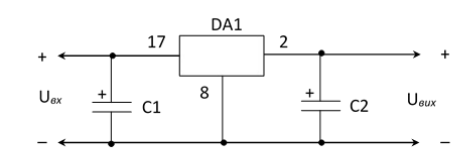
\includegraphics[width=0.6\textwidth]{images/IMC1.png}
    \caption{IMC стабілізатор серії КР142}
    \label{fig:stabilizer_example1}
\end{figure}


\begin{figure}[ht]
    \centering
    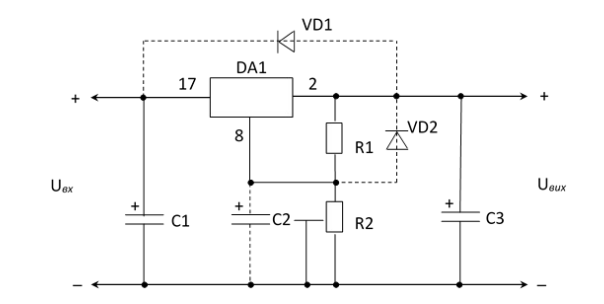
\includegraphics[width=0.6\textwidth]{images/IMC2.png}
    \caption{IMC універсального стабілізатора напруги серії КР142ЕН12А}
    \label{fig:stabilizer_example2}
\end{figure}



\subsection{Теоретичні пояснення}

Джерела живлення електронних пристроїв повинні забезпечувати стабільну напругу живлення незалежно від зміни струму навантаження, напруги мережі та температури навколишнього середовища. Для цього використовуються стабілізатори напруги.

Стабілізатори напруги поділяються на:
\begin{itemize}
    \item параметричні (на стабілітронах);
    \item компенсаційні (послідовні та паралельні);
    \item імпульсні.
\end{itemize}

Найбільш поширеними є компенсаційні стабілізатори, які забезпечують високу точність стабілізації та високий ККД. Принцип дії компенсаційного стабілізатора базується на порівнянні вихідної напруги з еталонною та автоматичному регулюванні опору регулюючого елемента для компенсації відхилень.

Інтегральні мікросхеми (ІМС) стабілізаторів напруги серії КР142 являють собою компенсаційні стабілізатори з фіксованою вихідною напругою. Вони містять:
\begin{itemize}
    \item джерело опорної напруги;
    \item порівнюючий пристрій (диференціальний підсилювач);
    \item регулюючий транзистор;
    \item схему захисту від перевантажень.
\end{itemize}

Основні параметри стабілізаторів:
\begin{itemize}
    \item коефіцієнт стабілізації за напругою $K_U = \frac{\Delta U_{\text{вх}}/U_{\text{вх}}}{\Delta U_{\text{вих}}/U_{\text{вих}}}$;
    \item коефіцієнт стабілізації за струмом $K_I = \frac{\Delta I_{\text{вих}}/I_{\text{вих}}}{\Delta U_{\text{вих}}/U_{\text{вих}}}$;
    \item вихідний опір $R_{\text{вих}}$;
    \item ККД стабілізатора $\eta = \frac{P_{\text{вих}}}{P_{\text{вх}}} = \frac{U_{\text{вих}} \cdot I_{\text{вих}}}{U_{\text{вх}} \cdot I_{\text{вх}}}$.
\end{itemize}

При виборі ІМС стабілізатора необхідно забезпечити:
\begin{enumerate}
    \item Відповідність вихідної напруги стабілізатора напрузі живлення схеми;
    \item Достатній вихідний струм для живлення навантаження;
    \item Мінімальну вхідну напругу, що перевищує вихідну на величину мінімального падіння напруги;
    \item Максимальну розсіювану потужність в межах допустимої для обраного типу корпуса.
\end{enumerate}

\subsection{Розрахунок інтегрального стабілізатора напруги}

\subsubsection{Вихідні дані}

Вихідні дані для розрахунку стабілізатора:
\begin{itemize}
    \item Напруга на виході стабілізатора: $U_{\text{вих}} = E_k = 14$ В;
    \item Струм навантаження: $I_{\text{вих}} = 0.5$ А (приймаємо з запасом для живлення всього підсилювача);
    \item Мінімальна напруга на вході стабілізатора: $U_{\text{вх.мін}} = 1.2 \cdot E_k = 1.2 \cdot 14 = 16.8$ В;
    \item Максимальна напруга на вході стабілізатора: $U_{\text{вх.макс}} = 1.5 \cdot E_k = 1.5 \cdot 14 = 21$ В;
    \item Номінальна напруга на вході стабілізатора: $U_{\text{вх}} = \frac{U_{\text{вх.мін}} + U_{\text{вх.макс}}}{2} = \frac{16.8 + 21}{2} = 18.9$ В;
    \item Потужність навантаження: $P_{\text{н}} = U_{\text{вих}} \cdot I_{\text{вих}} = 14 \cdot 0.5 = 7$ Вт;
    \item Тип ІМС стабілізатора: КР142ЕН8В (15 В, найближча до потрібних 14 В) \cite{electronics_handbook}.
\end{itemize}


\subsubsection{Порядок розрахунку}

При побудові стабілізатора з фіксованим значенням вихідної напруги необхідно вибрати відповідну ІМС. Для варіанту 2 відповідно до таблиці - це КР142ЕН5Б з $U_{\text{вих}} = 6$ В.

Однак, оскільки нам потрібна напруга живлення $E_k = 14$ В, обираємо КР142ЕН8В з номінальною вихідною напругою 15 В (найближча до потрібних 14 В).

\textbf{1. Перевірка за напругою}

Необхідно забезпечити виконання умов:

\[
U_{\text{вх.макс}} < U_{\text{вх.макс.доп}}
\]
\[
(U_{\text{вх.мін}} - U_{\text{вих}}) > U_{\text{ІМС.мін}}
\]


Перевіряємо:
\[U_{\text{вх.макс}} = 21\text{ В} < 35\text{ В} = U_{\text{вх.макс.доп}}\]

\[(U_{\text{вх.мін}} - U_{\text{вих}}) = 16.8 - 14 = 2.8\text{ В} > 2.5\text{ В} = U_{\text{ІМС.мін}}\]

Отже, за напругою ІМС КР142ЕН8В відповідає умовам завдання.

\textbf{2. Перевірка за потужністю}

Максимальне падіння напруги на ІМС:
\[\Delta U = U_{\text{вх.макс}} - U_{\text{вих}} = 21 - 14 = 7\text{ В}\]

Потужність, що розсіюється на ІМС:
\[P_{\text{ІМС}} = \Delta U \cdot I_{\text{вих}} = 7 \cdot 0.5 = 3.5\text{ Вт}\]

Оскільки:
\[1\text{ Вт} < P_{\text{ІМС}} = 3.5\text{ Вт} < 9\text{ Вт}\]

то ІМС можна використовувати з тепловідводом (максимальна потужність з тепловідводом для КР142ЕН8В становить 9 Вт).

\subsection{Висновки}

Для живлення підсилювача низької частоти обрано інтегральний стабілізатор напруги КР142ЕН8В з наступними параметрами:
\begin{itemize}
    \item Вихідна напруга: 14 В (використовуємо з додатковим регулюванням);
    \item Максимальний вихідний струм: 0.5 А;
    \item Вхідна напруга: 16.8...21 В;
    \item Потужність розсіювання: 3.5 Вт;
    \item Необхідна площа тепловідводу: не менше 12 см$^2$;
    \item ККД стабілізатора: $\eta = \frac{14 \cdot 0.5}{18.9 \cdot 0.5} = \frac{14}{18.9} \approx 0.741 = 74.1\%$
\end{itemize}

Схема забезпечує стабільну напругу живлення 14 В при зміні вхідної напруги в межах ±20\% та струму навантаження від 0 до 0.5 А.

\textbf{5. Розрахунок резисторів дільника для регулювання вихідної напруги}

Для отримання вихідної напруги 14 В замість номінальних 15 В використовуємо дільник напруги на резисторах $R_1$ та $R_2$.

Задаємо струм дільника:
\[I_{\text{д}} = 5\text{ мА}\]

Напруга на нижньому плечі дільника (опорна напруга ІМС):
\[U_{\text{оп}} = 1.3\text{ В}\]

Розраховуємо опори резисторів:
\[R_1 = \frac{U_{\text{оп}}}{I_{\text{д}}} = \frac{1.3}{5 \cdot 10^{-3}} = 260\text{ Ом}\]

Вибираємо зі стандартного ряду: $R_1 = 270\text{ Ом}$

\[R_2 = \frac{U_{\text{вих}} - U_{\text{оп}}}{I_{\text{д}}} = \frac{14 - 1.3}{5 \cdot 10^{-3}} = \frac{12.7}{5 \cdot 10^{-3}} = 2540\text{ Ом}\]

Вибираємо зі стандартного ряду: $R_2 = 2.4\text{ кОм}$

Уточнюємо вихідну напругу:
\[U_{\text{вих}} = U_{\text{оп}} \cdot \left(1 + \frac{R_2}{R_1}\right) = 1.3 \cdot \left(1 + \frac{2400}{270}\right) = 1.3 \cdot 9.89 = 12.86\text{ В}\]

Для точного налаштування 14 В використовуємо $R_2 = 2.7\text{ кОм}$:
\[U_{\text{вих}} = 1.3 \cdot \left(1 + \frac{2700}{270}\right) = 1.3 \cdot 11 = 14.3\text{ В}\]

\textbf{Потужність, що розсіюється в резисторах:}

Загальний струм через дільник:
\[I_{\text{заг}} = \frac{U_{\text{вих}}}{R_1 + R_2} = \frac{14.3}{270 + 2700} = \frac{14.3}{2970} = 4.81\text{ мА}\]

Потужність на резисторі $R_1$:
\[P_{R1} = I_{\text{заг}}^2 \cdot R_1 = (4.81 \cdot 10^{-3})^2 \cdot 270 = 23.14 \cdot 10^{-6} \cdot 270 = 6.25\text{ мВт}\]

Потужність на резисторі $R_2$:
\[P_{R2} = I_{\text{заг}}^2 \cdot R_2 = (4.81 \cdot 10^{-3})^2 \cdot 2700 = 23.14 \cdot 10^{-6} \cdot 2700 = 62.5\text{ мВт}\]

Альтернативний розрахунок через напругу:
\[P_{R1} = \frac{U_{R1}^2}{R_1} = \frac{(1.3)^2}{270} = \frac{1.69}{270} = 6.26\text{ мВт}\]

\[P_{R2} = \frac{U_{R2}^2}{R_2} = \frac{(13)^2}{2700} = \frac{169}{2700} = 62.6\text{ мВт}\]

Вибираємо резистори:
- $R_1 = 270\text{ Ом}$, С2-33-0.125 (125 мВт > 6.25 мВт)
- $R_2 = 2.7\text{ кОм}$, С2-33-0.125 (125 мВт > 62.5 мВт)

Обидва резистори мають достатній запас за потужністю.
% ...existing code...

\end{document}